Machine Learning methods, particularly Artificial Neural Networks (ANNs), have shown promising capabilities in solving a wide range of complex problems. Neural networks are a class of machine learning techniques that attempts to recognize underlying relationships in a set of data using a process similar to how the human brain works. An artificial neural network (ANN) is a machine learning algorithm inspired by biological neural networks. The nodes in each ANN communicate with one another via connections. A deep network can represent functions of increasing complexity by adding more layers and units within a layer.

\pagebreak

 \begin{figure}[h]
	\centering
	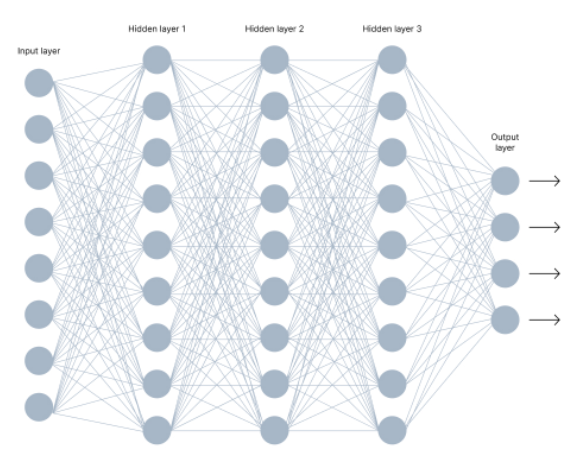
\includegraphics[width=0.6\textwidth]{figures/background/ANN.png}
	\captionsetup{labelformat=empty}
	\caption{\href{https://assets-global.website-files.com/5d7b77b063a9066d83e1209c/60d242974bcba9f8c670e03e_Group\%20806.jpg}
	{Neural Networks Architecture}}
\end{figure}

\subsubsection*{Artificial Neuron}
The fundamental building block of a neural network is a single neuron, which is also
 called a perceptron. More specifically, each neuron is a machine learning method that takes a set of features and their targets as input and tries to discover a line, plane, or hyperplane in two, three, or hyper-dimensional space that separates the classes. The sigmoid function is used to alter these characteristics.
 
 \begin{figure}[h]
	\centering
	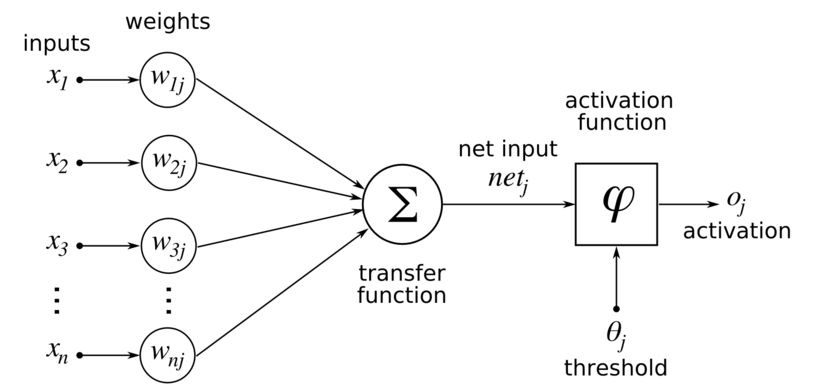
\includegraphics[width=0.6\textwidth]{figures/background/Neuron.png}
	\captionsetup{labelformat=empty}
	\caption{\href{https://commons.wikimedia.org/wiki/File:ArtificialNeuronModel_english.png}
	{Artificial Neuron}}
\end{figure}

Simple ANNs have an input layer and an output layer with zero to three hidden layers, whereas deep neural networks have no limit in the number of hidden layers. Multiple neurons make up a layer of a multilayer perceptron, and the input values as well as the bias values are assigned
during the training process.



\subsubsection*{Activation function}
The Activation function is used to determine whether or not the neuron will be activated. This means that it will use simpler mathematical operations to determine whether the neuron's input to the network is essential or not throughout the prediction phase. These mathematical functions are added to an artificial neural network to assist it in learning complex patterns in data. The reason that activation functions are essential parts of a ANN is that the combination of nonlinear activation functions from different neurons permits the network to approximate complex functions or distributions of data. Simpler, the most important feature of an activation function is to add non-linearity to a neural network. There are many activation functions, but here we show the most used functions.

 \begin{figure}[h]
	\centering
	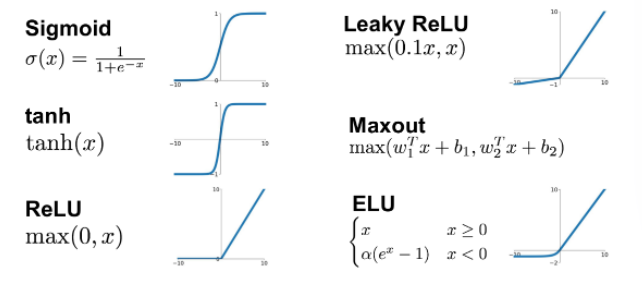
\includegraphics[width=0.6\textwidth]{figures/background/ActivationFunctions.png}
	\captionsetup{labelformat=empty}
	\caption{\href{https://datasciencepreparation.com/blog/articles/what-is-an-activation-function-what-are-commonly-used-activation-functions/}
	{Most common activation functions}}
\end{figure}

\subsubsection*{Loss Function}

One of the most important aspects of an ANN is the choice of the loss function \cite{The importance of the loss function in option valuation} . A loss function is incredibly simple at its core: It's a technique for determining how well your algorithm models your dataset. If the ANN predictions are completely incorrect, the loss function will return a higher value. Otherwise, it will return a lower value. However, minimizing the loss function doesn't necessarily mean that the prediction is getting closer to the desired results. There are some well-known categories of loss functions that may work on many simple ANN, but if the problem that the ANN has to solve is too complicated, it may need a custom loss function, that is special for the specific problem and ANN architecture. \\

In particular, the purpose of a loss function in an ANN is to adjust the weights and the bias during the training. If we could, we would find the perfect weights and bias for our ANN, but it has not yet been proven a formula that could do it. Therefore, these functions will try to find the adjustments, that are as close as to the perfect one's. \\

Pressingly, the loss function that is used is directly related to the activation function that is used in the neural network's output layer. Consider the output layer configuration to be a choice about the framing of the prediction problem, and the loss function selection to be the method for calculating the error for a given framing of the problem. The loss functions can be classified into two major categories depending upon the type of learning task we are dealing with Regression losses and Classification losses. In classification, we are trying to predict output from set of finite categorical values. Regression, on the other hand, deals with predicting a continuous value.

\subsubsection*{Back-propagation}

 \begin{figure}[h]
	\centering
	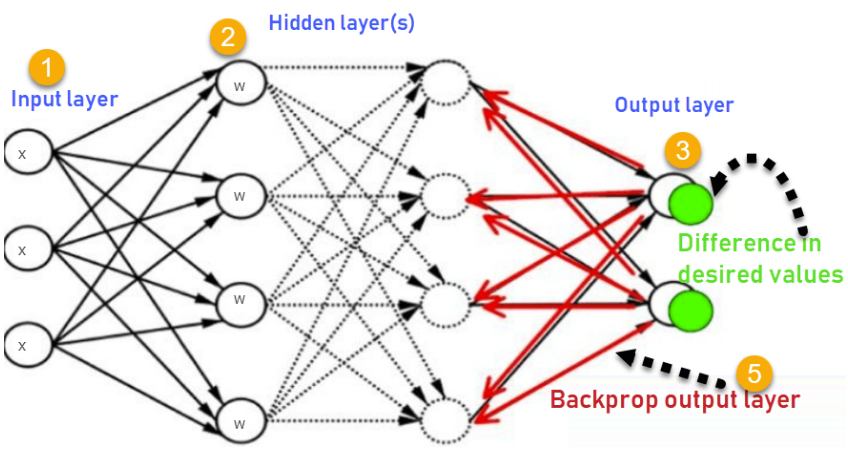
\includegraphics[width=0.8\textwidth]{figures/background/Backpropagation.png}
	\captionsetup{labelformat=empty}
	\caption{\href{https://www.guru99.com/images/1/030819_0937_BackPropaga1.png}
	{Backpropagation Algorithm}}
\end{figure}


The essence of neural net training is back-propagation. It is the practice of fine-tuning a neural net's weights based on the error rate obtained in the previous epoch. Proper weight tuning ensures lower error rates, increasing the model's reliability by increasing its generalization. \\

The back-propagation algorithm in neural networks computes the gradient of the loss function for a single weight using the chain rule. Unlike native direct computation, it efficiently computes one layer at a time. The back-propagation algorithm, allows the information from the cost to then flow backwards through the network, in order to compute the gradient. Back-propagation refers only to the method for computing the gradient, while another algorithm,
such as stochastic gradient descent, is used to perform learning using this gradient.

